\begin{figure}[H]
    \caption{An Example with Two Pieces}
    \label{fig:two_panels}
    \centering

	\subfloat[Here is one]{
	    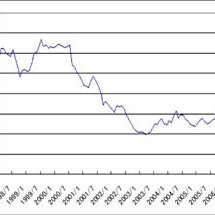
\includegraphics[width=3.0in]{fig/dummy_figure.jpg}
	 }
	\subfloat[Here is another]{
	    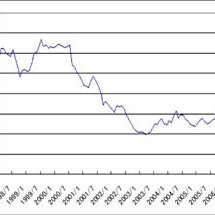
\includegraphics[width=3.0in]{fig/dummy_figure.jpg}
	 }
    \vspace{0.2cm}
    \begin{minipage}{0.95\textwidth} 
	{\footnotesize Now see how we can have two panels! \ldots
	\par
	}
	\end{minipage}
\end{figure}
